\begin{savequote}[6cm]
<< What is this place

Filled with so many wonders?

Casting its spell

That I am now under >>

\qauthor{Fluttershy, So Many Wonders}
\end{savequote}

\chapter{DomVision : Application au réseau local domestique}
\chaptertoc
Nous avons présenté dans le chapitre d'introduction le contexte fil rouge sur lequel cette thèse s'appuie. Ce chapitre permet de mettre en pratique la solution d'observation. DomVision est l'instanciation d'Astronef-Asteroid sur le réseau local domestique. Ainsi, en quelques composants et en plusieurs requêtes, nous arrivons à mettre en œuvre un système d'observation.

Dans ce chapitre, nous présentons les différents points de mise en application qui nous permettent de valider notre contribution dans son ensemble. En premier lieu, dans la section~\ref{sec:valid:domvision:systeme}, nous présentons comment nous nous sommes adapté au système observé. Ensuite, en section~\ref{sec:valid:domvision:requetes}, nous détaillons les requêtes que nous avons pu déployer grâce à l'expressivité d'Astral. Cela couvre la mise à jour de la base de données comme les requêtes de l'utilisateur. Enfin, en section~\ref{sec:valid:domvision:architecture} nous démontrons la flexibilité de notre solution en introduisant un nouvel opérateur capable d'établir des préférences sur les observations.

\section{Adaptation au système observé}\label{sec:valid:domvision:systeme}
Dans cette section, nous analysons le système au sens où nous l'avons décrit jusqu'ici dans Astronef et Asteroid. Nous devons modéliser le système pour en extraire son schéma qui permet de représenter le catalogue dans la base d'Asteroid. Puis nous nous intéressons aux données temps-réel. En enfin, nous présentons les flux à notre disposition dans ce réseau.

\subsection{Le schéma du système}
Nous présentons ici la vision que nous avons du système que nous observons. Il est important de voir que cette vision ne doit pas être liée aux sources de données disponibles. Elle a pour but de refléter l'interprétation des experts souhaitant observer le système.

Pour chaque concept, il est nécessaire de pouvoir identifier les objets du système pour pouvoir leur associer nos observations. Ainsi, nous détaillons les attributs permettant de désigner un objet de façon unique. Toutefois, dans la pratique, les données collectées sont partielles et ces attributs peuvent être absents. Ces inconsistances peuvent être minimisées par l'utilisation d'heuristiques. Les conséquences de telles inconsistances seraient la création de plusieurs entrées dans le catalogue qui représentent le même objet du système.

Chaque concept est caractérisé par un ensemble de propriétés \textit{statiques}, relatives à sa description, et \textit{stables}, relatives à son état. Les données volatiles sont présentées dans la section suivante. Nous définissons ici trois concepts principaux : les équipements, les applications et les interfaces réseau.

\subsubsection{Équipements}
La notion d'équipement est une vision orientée utilisateur. En effet, un \textit{équipement} est un châssis physique. Les équipements virtuels ne sont pas représentés. Ce choix permet de représenter à l'utilisateur les appareils qu'il est capable de voir et de manipuler (débrancher par exemple). Quelques exemples : \textit{Livebox}, \textit{STB}\footnote{Set Top Box : Boitier connecté à une télévision pour fournir les services de partage de contenus, de télévisions, VOD...}, Ordinateurs, Tablettes, Disques durs réseaux.

\textbf{Identification} : un équipement \textit{peut} avoir un \textit{numéro de série} unique. L'utilisation des interfaces ou applications liées permet un moyen alternatif.

\subsubsection{Applications}
Nous désignons par \textit{application} un programme instancié sur un des équipements. À un \textit{équipement} est associé plusieurs \textit{applications}. Les \textit{applications} permettent d'effectuer des tâches sur leurs équipements respectifs. Une \textit{application} en exécution a un état. Dans cette expérimentation, nous ne considérons que \textit{actif} et \textit{inactif}. Plusieurs autres statuts pourraient être utilisés comme \textit{suspendu} ou \textit{gelé}. Notons que la détermination des statuts est généralement complexe, car le système fournit rarement des données précises à ce sujet puisque cela consiste en un autodiagnostic\footnote{L'utilisation d'inférences de haut niveau comme vu en section~\ref{sec:rw:supervision:contexte} peut devenir intéressante dans ces cas.}. Quelques exemples : Partage de contenu, Agent d'administration, Gestion d'impression. Une \textit{application} a un \textit{nom}, une \textit{description} textuelle et potentiellement un \textit{type}.

\textbf{Identification} : une application \textit{peut} fournir un \textit{nom} unique par l'utilisation d'un \textit{UUID}, par exemple. Alternativement, nous pouvons exploiter l'unicité de son \textit{type}. Par exemple, il n'existe qu'une application de passerelle internet sur le réseau domestique.

\subsubsection{Interfaces réseaux}
Les \textit{interfaces réseaux} sont moins sujets à interprétation que les deux concepts précédents. Une \textit{interface réseau} représente un point de connexion que possède un \textit{équipement} vers le réseau domestique. Nous supposons que cette interface est une interface \textit{MAC}\footnote{Permettant des interfaces \textit{IP} et \textit{Zigbee} potentiellement}. Elle possède un \textit{nom} système unique pour l'équipement, un type (wifi, Ethernet), ainsi qu'une adresse \textit{MAC} considéré unique sur le réseau et d'autres adresses comme \textit{IPv4} ou \textit{v6}.

\textbf{Identification} : seule l'adresse \textit{MAC} garantit l'unicité. Si elle n'est pas renseignée, l'adresse \textit{IP} peut être utilisé comme moyen alternatif.

\subsubsection{Concepts supplémentaires possibles}
Ayant une modélisation des concepts principaux du réseau local domestique, nous pouvons maintenant ajouter des concepts supplémentaires. Bien que nous ne les utilisons pas dans la suite de ce chapitre, il est intéressant de les garder à l'esprit.

Par exemple, pour développer la topologie du réseau, les \textit{liens} relient deux interfaces réseaux. Les \textit{chemins} sont composés de \textit{liens} réseaux. Et les \textit{canaux de transport} peuvent utiliser un \textit{chemin} pour aussi relier deux \textit{applications}. Toutefois, la collecte de ces informations est soumise à des contraintes de mise en œuvre plus technique comme l'utilisation de protocoles \textit{LLTD} ou \textit{IEEE P1905.1}.

\subsection{Les données volatiles intéressantes}
Comme défini au chapitre~\ref{chap:contrib:asteroid}, les données \textit{volatiles} sont des données temps réel que nous souhaitons archiver en vue d'une analyse a posteriori. La surveillance de l'état d'un réseau domestique passe par l'observation de métriques de charge. Ces dernières sont par exemple visualisées sur des graphiques afin de détecter des comportements anormaux.

Pour les équipements, nous surveillons la charge processeur utilisé (en \%) et mémoire occupée (en ko). Pour les interfaces réseau, le débit est un bon indicateur de son état. Au besoin, d'autres métriques plus spécifiques peuvent être enregistrées comme : la latence ou la gigue d'une interface réseau.

Nous souhaitons observer des changements d'état. L'état est caractérisé par un modèle qui contient des données de différentes dynamiques telles que des données de description (\textit{statique}), de configuration (\textit{stable}) et de fonctionnement (périodique ou imprévisible). Par exemple, nous pouvons surveiller les changements de topologie du réseau. Pour cela, nous observons les changements d'adresse \textit{IP} des interfaces, ou de \textit{statut} des équipements, applications et interfaces.

Désormais, nous avons formalisé notre représentation du réseau domestique. Analysons maintenant les données produites par le réseau domestique et pour pouvoir les intégrer à cette représentation.

\subsection{Les données disponibles}\label{sec:valid:domvision:systeme:data}
Dans notre mise en œuvre, nous utilisons le protocole \textit{UPnP} largement répandu dans le réseau domestique. Ce protocole permet d'annoncer un \textit{Device}\footnote{Attention au vocabulaire utilisé par le protocole. Un \textit{device} UPnP est en réalité une \textit{application} déployée sur un \textit{équipement}.}. Ce \textit{Device} exposant des \textit{Services} qui contiennent des \textit{Actions}, il est possible de les consulter à distance. Les \textit{Devices} répondent à des profils standards.

De fait, l'annonce des \textit{Device} \textit{UPnP} sur le réseau produit un flux de données \begin{center}\textit{UPnPStatus}(uuid, ip, type, friendlyName, status, $\t$).\end{center} Ce flux indique que le \textit{device UPnP} annoncé avec l'IP \textit{ip}, ayant pour identifiant unique \textit{uuid}, pour profil \textit{type} et pour description textuelle \textit{friendlyName} a changé son statut au temps $\t$ pour \textit{status}.

Nous avions exploré en section~\ref{sec:rw:supervision:administration} que les protocoles et agents d'administrations pouvaient être de bons interlocuteurs pour fournir des données. Dans le monde \textit{UPnP}, il existe le profil \textit{DeviceManagement} capable de fournir des données intéressantes. Le tableau~\ref{tab:valid:domvision:upnpdm} indique les données que nous pouvons exploiter. Les flux produits ont, en plus des paramètres, les attributs \textit{uuid} correspondants à l'identifiant \textit{UPnP} de l'agent, ainsi que le \textit{timestamp} d'émission $\t$.

\begin{table}[ht]
\centering
\begin{tabular}{|m{0.25\textwidth}|>{\ttfamily}m{0.25\textwidth}|m{.4\textwidth}|} \bottomrule
\rowcolor{hypcolor} Nom du flux & \rm Paramètre & Description du paramètre\\ \hline
\multicolumn{3}{|c|}{/UPnP/DM/DeviceInfo/PhysicalDevice/} \\\hline
Serial & {SerialNumber} & Numéro de série de l'équipement\\\hline
\multirow{3}{*}{NetworkInterface} & {SystemName} & Nom de l'interface réseau\\\cline{2-3}
& {MACAddress} & Adresse MAC de l'interface\\\cline{2-3}
& InterfaceType & Type de l'interface \\\hline
\multicolumn{3}{|c|}{/UPnP/DM/Configuration/} \\\hline
\multirow{2}{*}{IPInterface} & SystemName & Nom de l'interface réseau \\\cline{2-3}
& IPv4Address & Adresse \textit{IPv4} de l'interface \\ \hline
\multicolumn{3}{|c|}{/UPnP/DM/Monitoring/} \\\hline
\multirow{2}{*}{OperatingSystem} & CPUUsage & Charge actuelle du processeur\\\cline{2-3}
& MemoryUsage & Charge actuelle de la mémoire\\ \hline
\multirow{3}{*}{IPUsage} & SystemName & Nom de l'interface réseau\\ \cline{2-3}
& TotalBytesSent & Nombre d'octets envoyés \\\cline{2-3}
& TotalBytesReceived & Nombre d'octets reçus \\ \toprule
\end{tabular}
\caption{Listes des flux intéressant fournis par le profil UPnP-DM}\label{tab:valid:domvision:upnpdm}
\end{table}

\subsection{Les sources Astronef}
Nous avons conçu un composant spécifique pour la formation du flux \textit{UPnPStatus}. Ce composant n'a pas de paramètre et fournit le service \textit{Source}, comme présenté dans le chapitre~\ref{chap:contrib:astronef}, avec comme attributs ceux mentionnés dans la section~\ref{sec:valid:domvision:systeme:data}. Son fonctionnement est événementiel.

Pour la communication sur \textit{UPnP-DM}, nous souhaitons créer un composant réutilisable. Nous avons conçu un composant générique capable d'interroger tous les nœuds du modèle de données d'\textit{UPnP-DM} et de fonctionner de manière événementielle ou périodique. Or, le protocole possède un mécanisme de notification sur changement de valeur sur certaines variable d'état (propriété \textit{EventOnChange}~\cite{UPnP:DM2}). Un mécanisme spécifique a été créé pour qu'un composant externe puisse indiquer à la source de collecter les données. Enfin, le composant doit itérer si nécessaire pour récupérer toutes les instances (\#) d'un chemin et envoyer l'ensemble des données dans un seul \textit{batch}, comme prévu dans Astral. L'ensemble des paramètres de cette source est présenté dans la table~\ref{tab:valid:domvision:dmsource}.

\begin{table}[ht]
    \centering
    \begin{tabular}{cl}
        paramètre & description \\ \midrule
        path & Chemin d'accès aux données \\
        parameters & Liste CSV des paramètres souhaités \\
        period & Période de mise à jour du flux (optionnel) \\
        channel & Canal interne d'événement à souscrire (optionnel)
    \end{tabular}
    \caption{Paramètres du composant \textit{DMSource}}\label{tab:valid:domvision:dmsource}
\end{table}

Nous construisons périodiquement les flux \textit{OperatingSystem} et \textit{IPUsage} qui contiennent des données \textit{périodiques}. Les autres flux sont des données \textit{imprévisibles} et sont construits à chaque arrivée de \textit{Device} de ce profil. Pour cela, nous formons la requête $\sigma_{status=active\wedge type=dm}$ \textit{UPnPStatus}\footnote{D'autres requêtes pourraient être utilisées en exploitant les mécanismes de notification de changement de variable d'état.}. Cette requête est injectée dans le puits \textit{SourceNotifier} afin de notifier les \textit{Sources} qui se sont inscrites. Ici, toutes les instances de \textit{DMSource} souhaitant être notifiées le sont par le canal d'événement \textit{DM}. Nous pouvons voir la synergie entre les requêtes déployées et les différent composants et services de notre intergiciel. En effet, nous avons réussi à coordonner les deux mécanismes présentés en section~\ref{sec:rw:supervision:administration} via l'utilisation de requêtes.

Nous avons vu la représentation du système, les données intéressantes, et la façon d'obtenir ces données. Nous présentons désormais des exemples de requêtes que nous posons au système d'observation pour démontrer son expressivité.
\section{Expressivité du système d'observation}\label{sec:valid:domvision:requetes}
\subsection{Entretien du modèle descriptif}
\subsection{Historisation des paramètres}
\subsection{Formations d'alertes}
\section{Architecture interne d'Astronef}\label{sec:contrib:astronef:architecture}
Dans cette section, nous détaillons les éléments d'architecture que nous avons mis en œuvre pour permettre à une requête Astral d'être instanciée en un processus de traitement. Nous abordons premièrement les principes architecturaux utilisés. Ensuite, nous détaillons les différents composants utilisés dans Astronef. Enfin, nous présentons notre méthode extensible de construction de plan par l'utilisation d'un système de règles.
\subsection{Choix d'architecture logicielle}
Avant de détailler l'architecture de notre système de traitement de requêtes continues, nous allons d'abord présenter le paradigme architectural dans lequel nous allons mettre en œuvre Astronef. Nous présentons premièrement et brièvement les architectures à services. Puis, nous détaillons les principes des architectures à composants orientés services que nous utilisons par la suite.
\subsubsection{Architecture à service}
Les architectures à services permettent aux applications d'être assemblés sous forme de blocs réutilisables : des \textit{services}. Un \textit{service} est définit par une spécification (ou \textit{description}, ou \textit{contrat}), qui décrit sa syntaxe, son comportement, sa sémantique ainsi que sa dépendance aux autres services. Dans les architectures à services, les services interagissent via un patron récurrent d'interaction (fig~\ref{fig:contrib:astronef:services}). 
\begin{figure}[ht]
    \centering
    \includegraphics[width=0.7\textwidth]{contrib-astronef-services}
    \caption{Patron d'interaction de service}\label{fig:contrib:astronef:services}
\end{figure}
Un fournisseur de service va publier sa spécification à un registre. Un consommateur de service découvre le service fournit par une requête sur le registre. Enfin, le consommateur et le fournisseur se connectent. Le point clé est que la résolution est faite à l'exécution.

\subsubsection{Architecture à composants orientés services}
Le modèle d'architecture à composants orientés services~\cite{Cervantes:servicecomponent} permet la mise en œuvre d'applications à base de services dans le paradigme de la programmation par composants. Le principe est de séparer les mécanismes des architectures à services du code implémentant le comportement du service fournit. Ainsi, les principes d'un tel modèle sont :
\begin{itemize}
    \item Un service est une fonctionnalité fournie.
    \item Un service est caractérisé par sa spécification.
    \item Les composants implémentent des spécifications de services, qui peuvent eux-mêmes dépendre, du fait de leurs implémentations, d'autres services.
    \item Les patrons d'interactions de services sont utilisés pour résoudre les dépendances de services à l'exécution.
    \item Les compositions sont décrites en terme de spécifications de services.
    \item Tout composant peut se substituer par un autre si les spécifications de services sont identiques.
\end{itemize}
Le modèle combine les idées de composants et de services. De plus, en s'inspirant des modèles tels que Fractal~\cite{Bruneton:fractal}, chaque composant possède un ensemble de propriétés (ou attributs) configurables. Nous obtenons aussi le pouvoir d'instancier (grâce aux fabriques) des composants à partir de configurations.

\begin{figure}[ht]
    \centering
    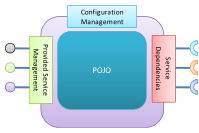
\includegraphics[width=0.5\textwidth]{contrib-astronef-ipojo}
    \caption{Un composant iPojo}\label{fig:contrib:astronef:ipojo}
\end{figure}
La figure~\ref{fig:contrib:astronef:ipojo} représente un composant dans l'implémentation \textit{iPojo}~\cite{Escoffier:ipojo}. Le code du composant (le \textit{POJO}, \textit{Plain Old Java Object}) est embarqué dans un conteneur auxquels sont accrochés des gestionnaires. Les trois couramment utilisés sont les gestionnaires de dépendances, de production de service, et de configuration. Ainsi, un composant peut s'exposer sur un registre, tout en dépendant d'autres services et en étant configurable.

\subsection{Les composants et services d'Astronef}
L'architecture d'Astronef est entièrement dirigé par les approches de composants orientés services. De multiples composants sont créés et instantiés, pour former une requête. Afin de pouvoir exécuter les requêtes, nous définissons trois services centraux :
\begin{itemize}
	\item[\textbf{Les services \textit{EventProcessor}}] ont deux primitives, l'une exécute une tâche, l'autre indique les \textit{EventProcessors} devant être exécutés avant soi-même.
	\item[\textbf{Le service \textit{Scheduler}}] permet la planification. Ses primitives permettent aux différents \textit{EventProcessor} d'exprimer leur volonté de s'exécuter. Ce service établit l'ordonnancement de ces demandes en fonction des contraintes des \textit{EventProcessor}s.
	\item[\textbf{Le service \textit{QueryRuntime}}] permet d'exécuter une requête. Il est lié à un \textit{Scheduler} et utilise la primitive \textit{next} de celui-ci pour connaître la prochaine tâche à exécuter.
\end{itemize}

Nous adoptons l'approche émise par~\cite{Carney:scheduling} en gérant l'ordonnancement par un service externes aux opérateurs, comme présenté dans la section~\ref{sec:rw:sgfd:infra}. Maintenant que nous avons vu les différents services nécessaire à l'exécution. Nous avons plusieurs types de composants que nous pouvons instantier par des services de fabriques :
\begin{itemize}
	\item[\textbf{Les flux ou relations} (entités)] : Fournissent les primitives nécessaires à leur manipulation par Astral. Ces entités servent de résultats intermédiaires (ou de tampons). De plus, ils permettent un service de notification. En cas de changement, les \textit{EventProcessor} abonnés sont notifiés. Ainsi, ces composants nécessitent un \textit{Scheduler} pour demander l'exécution de leurs abonnés.
	\item[\textbf{Les sources}] : Une source nécessite une entité qu'elle alimente grâce aux données issues d'origines diverses (protocoles réseaux, fichiers,...). Ce composant peut nécessiter le \textit{Scheduler} pour, entre autres, notifier sa fin de vie ce qui peut engendrer la fin de vie de la requête.
	\item[\textbf{Les opérateurs}] : Nécessitent $n$ entités en lecture, et une autre particulière en écriture. Ce composant doit fournir le service \textit{EventProcessor}. Les implémentations des opérateurs bloquants peuvent faire appel au \textit{Scheduler} pour planifier des exécutions ponctuelles.
	\item[\textbf{Les puits}] : Nécessitent une entité en lecture. Ce composant fournit le service \textit{EventProcessor} et doit être non-bloquant.
\end{itemize}

Ainsi pour créer une requête : l'utilisateur de l'intergiciel doit fournir un ou plusieurs composants sources et un composant puit. Par la suite, il demande à Astronef de lui instantier ses sources et son puit en configurant les composants selon sa volonté. Enfin, il spécifie l'expression algébrique liant les sources au puit.

\subsubsection{De l'importance de la réutilisation}
\textit{Astronef} permet une grande flexibilité grâce aux composants orientés services. Tout d'abord, chaque composant peut être configuré tout en gérant son cycle de vie, ce qui permet de réutiliser le même module pour plusieurs usages. Par exemple, supposons l'existence d'une source capable de récupérer une information périodiquement sur un dispositif $D$ via un protocole donné. Cette source peut être utilisée pour plusieurs requêtes sous différentes instances en ayant plusieurs configurations : différents dispositifs ou périodes d'acquisitions.

Cette abstraction sous forme de services permet surtout la substitution. En effet, nous pouvons remplacer tout composant par un autre supportant le même service. Nous utilisons ce principe pour sélectionner les meilleurs composants pour remplir le plus efficacement leurs rôles. De plus, l'utilisateur peut apporter ses propres implémentations pour étendre les capacités de l'intergiciel.

\section{Conclusion}
Après 20 années de recherche, la gestion de flux de données devient désormais suffisamment mature pour être appliqué massivement. Plusieurs produits commerciaux sont d'ailleurs maintenant utilisés en production. Toutefois, nous pouvons nous rendre compte que la complexité théorique de ces systèmes a été sous-estimé. De nombreux modèles ont été décrit pour représenter les flux de données et leurs traitements. Ces modèles sont encore remis en questions aujourd'hui au fur et à mesure des applications concrètes. 

Nous avons vu que le problème d'avoir une bonne connaissance du modèle et du comportement théorique des SGFD est crucial. En l'état, l'intégration des supports persistants reste ad-hoc et assisté par l'utilisateur. Un fonctionnement intégré avec une modélisation générique capable de gérer les deux modes d'interrogations de façon unifiée est donc indispensable pour manipuler correctement flux et relations persistantes. Similairement, les contributions sur l'optimisation de traitement des requêtes sont encore principalement ponctuelles. Afin d'appliquer un traitement efficace pour toute requête, il est nécessaire d'avoir une bonne connaissance théorique du traitement.

Notre contribution technique se concentrera sur trois points principaux :
\begin{itemize}
 \item[\textbf{Modélisation}] : Création d'Astral, algèbre de traitement des requêtes continues sur flux et relations temporelles. Nous accorderons de l'importance sur la prise en compte des problèmes relevés en section~\ref{sec:rw:sgfd:modeles:synthese}. Cette algèbre sera présenté dans le chapitre~\ref{chap:contrib:astral}
 \item[\textbf{Exécution}] : Mise en œuvre de l'intergiciel Astronef pour construire et exécuter efficacement une requête exprimée avec l'algèbre Astral. Ainsi, à partir d'une requête algébrique, il est possible de sélectionner le plan de requête qui semble le plus efficace grâce aux connaissances accumulés. Cette mise en œuvre sera développée dans le chapitre~\ref{chap:contrib:execution}.
 \item[\textbf{Persistance}] : Conception de l'extension Asteroid permettant l'intégration des requêtes continues sur flux et des requêtes sur support relationnel persistant. Ceci permettra de gérer la représentation du système observé ainsi que l'historisation des données dynamiques. Le support mathématique de cette intégration sera supporté par Astral et sa mise en œuvre par Astronef. Cette intégration sera effectuée dans le chapitre~\ref{chap:contrib:persistance}.
\end{itemize}

Grâce à ces contributions, il deviendra possible de mettre en œuvre un système d'observation générique applicable sur tout type de données. L'utilisateur devra exprimer des requêtes dans le langage algébrique Astral. Une fois ces requêtes écrites, nous serons garanti de leur mise en œuvre. Le tableau~\ref{tab:rw:contrib} résume l'ensemble des points d'analyses que nous nous étions fixés en section~\ref{sec:rw:supervision:criteres}.
\begin{table}[!ht]
\criteretabDonnee
    {Relationnel dérivé. Nous réutilisons les principes utilisés dans la gestion de flux et des bases de données.}
    {\good Modèle entité-relation augmenté pour supporter les flux.}
    {\good Requêtes sur tout type de données (flux, relations).}
\criteretabTraitement
    {\good Continue, Instantannée, Mixte}
    {\good Utilisation des requêtes continues des SGFD en tant qu'intégrateur.}
    {\meh Astral : langage de requête algébrique. Un langage purement déclaratif reste toutefois dérivable de ces fondations théoriques.}
    {\good Relationnel avec support \textbf{intégré} du dynamisme des données.}
\criteretabAdaptabilite
    {\good Spécification du modèle du système ainsi que des requêtes d'intégration (algébriques).}
    {\meh Pour l'analyse, la gestion de données multi-dimensionnelles des entrepôts utilisés est utilisé. Pour l'interrogation continue, utilisation d'un opérateur de préférences sur les flux.}
    {\good Infrastructure générique capable de supporter l'ajout d'opérateurs avec plusieurs implémentations.}
    {\good Héritage de l'efficacité des flux de données. Sélection du meilleur plan d'exécution pour chaque requête. Héritage des supports de grands volumes grâce aux entrepôts.}
\caption{Résumé de notre contribution selon nos critères}\label{tab:rw:contrib}
\end{table}
